%% bare_conf.tex
%% V1.4b
%% 2015/08/26
%% by Michael Shell
%% See:
%% http://www.michaelshell.org/
%% for current contact information.
%%
%% This is a skeleton file demonstrating the use of IEEEtran.cls
%% (requires IEEEtran.cls version 1.8b or later) with an IEEE
%% conference paper.
%%
%% Support sites:
%% http://www.michaelshell.org/tex/ieeetran/
%% http://www.ctan.org/pkg/ieeetran
%% and
%% http://www.ieee.org/

%%*************************************************************************
%% Legal Notice:
%% This code is offered as-is without any warranty either expressed or
%% implied; without even the implied warranty of MERCHANTABILITY or
%% FITNESS FOR A PARTICULAR PURPOSE! 
%% User assumes all risk.
%% In no event shall the IEEE or any contributor to this code be liable for
%% any damages or losses, including, but not limited to, incidental,
%% consequential, or any other damages, resulting from the use or misuse
%% of any information contained here.
%%
%% All comments are the opinions of their respective authors and are not
%% necessarily endorsed by the IEEE.
%%
%% This work is distributed under the LaTeX Project Public License (LPPL)
%% ( http://www.latex-project.org/ ) version 1.3, and may be freely used,
%% distributed and modified. A copy of the LPPL, version 1.3, is included
%% in the base LaTeX documentation of all distributions of LaTeX released
%% 2003/12/01 or later.
%% Retain all contribution notices and credits.
%% ** Modified files should be clearly indicated as such, including  **
%% ** renaming them and changing author support contact information. **
%%*************************************************************************


% *** Authors should verify (and, if needed, correct) their LaTeX system  ***
% *** with the testflow diagnostic prior to trusting their LaTeX platform ***
% *** with production work. The IEEE's font choices and paper sizes can   ***
% *** trigger bugs that do not appear when using other class files.       ***                          ***
% The testflow support page is at:
% http://www.michaelshell.org/tex/testflow/

\documentclass[conference]{IEEEtran}

\usepackage{graphicx}
\usepackage{color}
\usepackage{soul}
\usepackage{todonotes}
\usepackage{hyperref}
\usepackage{amsmath}
%\usepackage{fixltx2e}
%\usepackage{xcolor}
%\usepackage{morefloats}
%\usepackage{amsmath}

% Some Computer Society conferences also require the compsoc mode option,
% but others use the standard conference format.
%
% If IEEEtran.cls has not been installed into the LaTeX system files,
% manually specify the path to it like:
%\documentclass[conference]{../sty/IEEEtran}

% Some very useful LaTeX packages include:
% (uncomment the ones you want to load)


% *** MISC UTILITY PACKAGES ***
%
%\usepackage{ifpdf}
% Heiko Oberdiek's ifpdf.sty is very useful if you need conditional
% compilation based on whether the output is pdf or dvi.
% usage:
% \ifpdf
%   % pdf code
% \else
%   % dvi code
% \fi
% The latest version of ifpdf.sty can be obtained from:
% http://www.ctan.org/pkg/ifpdf
% Also, note that IEEEtran.cls V1.7 and later provides a builtin
% \ifCLASSINFOpdf conditional that works the same way.
% When switching from latex to pdflatex and vice-versa, the compiler may
% have to be run twice to clear warning/error messages.






% *** CITATION PACKAGES ***
%
%\usepackage{cite}
% cite.sty was written by Donald Arseneau
% V1.6 and later of IEEEtran pre-defines the format of the cite.sty package
% \cite{} output to follow that of the IEEE. Loading the cite package will
% result in citation numbers being automatically sorted and properly
% "compressed/ranged". e.g., [1], [9], [2], [7], [5], [6] without using
% cite.sty will become [1], [2], [5]--[7], [9] using cite.sty. cite.sty's
% \cite will automatically add leading space, if needed. Use cite.sty's
% noadjust option (cite.sty V3.8 and later) if you want to turn this off
% such as if a citation ever needs to be enclosed in parenthesis.
% cite.sty is already installed on most LaTeX systems. Be sure and use
% version 5.0 (2009-03-20) and later if using hyperref.sty.
% The latest version can be obtained at:
% http://www.ctan.org/pkg/cite
% The documentation is contained in the cite.sty file itself.






% *** GRAPHICS RELATED PACKAGES ***
%
\ifCLASSINFOpdf
  % \usepackage[pdftex]{graphicx}
  % declare the path(s) where your graphic files are
  % \graphicspath{{../pdf/}{../jpeg/}}
  % and their extensions so you won't have to specify these with
  % every instance of \includegraphics
  % \DeclareGraphicsExtensions{.pdf,.jpeg,.png}
\else
  % or other class option (dvipsone, dvipdf, if not using dvips). graphicx
  % will default to the driver specified in the system graphics.cfg if no
  % driver is specified.
  % \usepackage[dvips]{graphicx}
  % declare the path(s) where your graphic files are
  % \graphicspath{{../eps/}}
  % and their extensions so you won't have to specify these with
  % every instance of \includegraphics
  % \DeclareGraphicsExtensions{.eps}
\fi
% graphicx was written by David Carlisle and Sebastian Rahtz. It is
% required if you want graphics, photos, etc. graphicx.sty is already
% installed on most LaTeX systems. The latest version and documentation
% can be obtained at: 
% http://www.ctan.org/pkg/graphicx
% Another good source of documentation is "Using Imported Graphics in
% LaTeX2e" by Keith Reckdahl which can be found at:
% http://www.ctan.org/pkg/epslatex
%
% latex, and pdflatex in dvi mode, support graphics in encapsulated
% postscript (.eps) format. pdflatex in pdf mode supports graphics
% in .pdf, .jpeg, .png and .mps (metapost) formats. Users should ensure
% that all non-photo figures use a vector format (.eps, .pdf, .mps) and
% not a bitmapped formats (.jpeg, .png). The IEEE frowns on bitmapped formats
% which can result in "jaggedy"/blurry rendering of lines and letters as
% well as large increases in file sizes.
%
% You can find documentation about the pdfTeX application at:
% http://www.tug.org/applications/pdftex





% *** MATH PACKAGES ***
%
%\usepackage{amsmath}
% A popular package from the American Mathematical Society that provides
% many useful and powerful commands for dealing with mathematics.
%
% Note that the amsmath package sets \interdisplaylinepenalty to 10000
% thus preventing page breaks from occurring within multiline equations. Use:
%\interdisplaylinepenalty=2500
% after loading amsmath to restore such page breaks as IEEEtran.cls normally
% does. amsmath.sty is already installed on most LaTeX systems. The latest
% version and documentation can be obtained at:
% http://www.ctan.org/pkg/amsmath





% *** SPECIALIZED LIST PACKAGES ***
%
%\usepackage{algorithmic}
% algorithmic.sty was written by Peter Williams and Rogerio Brito.
% This package provides an algorithmic environment fo describing algorithms.
% You can use the algorithmic environment in-text or within a figure
% environment to provide for a floating algorithm. Do NOT use the algorithm
% floating environment provided by algorithm.sty (by the same authors) or
% algorithm2e.sty (by Christophe Fiorio) as the IEEE does not use dedicated
% algorithm float types and packages that provide these will not provide
% correct IEEE style captions. The latest version and documentation of
% algorithmic.sty can be obtained at:
% http://www.ctan.org/pkg/algorithms
% Also of interest may be the (relatively newer and more customizable)
% algorithmicx.sty package by Szasz Janos:
% http://www.ctan.org/pkg/algorithmicx




% *** ALIGNMENT PACKAGES ***
%
%\usepackage{array}
% Frank Mittelbach's and David Carlisle's array.sty patches and improves
% the standard LaTeX2e array and tabular environments to provide better
% appearance and additional user controls. As the default LaTeX2e table
% generation code is lacking to the point of almost being broken with
% respect to the quality of the end results, all users are strongly
% advised to use an enhanced (at the very least that provided by array.sty)
% set of table tools. array.sty is already installed on most systems. The
% latest version and documentation can be obtained at:
% http://www.ctan.org/pkg/array


% IEEEtran contains the IEEEeqnarray family of commands that can be used to
% generate multiline equations as well as matrices, tables, etc., of high
% quality.




% *** SUBFIGURE PACKAGES ***
%\ifCLASSOPTIONcompsoc
%  \usepackage[caption=false,font=normalsize,labelfont=sf,textfont=sf]{subfig}
%\else
%  \usepackage[caption=false,font=footnotesize]{subfig}
%\fi
% subfig.sty, written by Steven Douglas Cochran, is the modern replacement
% for subfigure.sty, the latter of which is no longer maintained and is
% incompatible with some LaTeX packages including fixltx2e. However,
% subfig.sty requires and automatically loads Axel Sommerfeldt's caption.sty
% which will override IEEEtran.cls' handling of captions and this will result
% in non-IEEE style figure/table captions. To prevent this problem, be sure
% and invoke subfig.sty's "caption=false" package option (available since
% subfig.sty version 1.3, 2005/06/28) as this is will preserve IEEEtran.cls
% handling of captions.
% Note that the Computer Society format requires a larger sans serif font
% than the serif footnote size font used in traditional IEEE formatting
% and thus the need to invoke different subfig.sty package options depending
% on whether compsoc mode has been enabled.
%
% The latest version and documentation of subfig.sty can be obtained at:
% http://www.ctan.org/pkg/subfig




% *** FLOAT PACKAGES ***
%
%\usepackage{fixltx2e}
% fixltx2e, the successor to the earlier fix2col.sty, was written by
% Frank Mittelbach and David Carlisle. This package corrects a few problems
% in the LaTeX2e kernel, the most notable of which is that in current
% LaTeX2e releases, the ordering of single and double column floats is not
% guaranteed to be preserved. Thus, an unpatched LaTeX2e can allow a
% single column figure to be placed prior to an earlier double column
% figure.
% Be aware that LaTeX2e kernels dated 2015 and later have fixltx2e.sty's
% corrections already built into the system in which case a warning will
% be issued if an attempt is made to load fixltx2e.sty as it is no longer
% needed.
% The latest version and documentation can be found at:
% http://www.ctan.org/pkg/fixltx2e


%\usepackage{stfloats}
% stfloats.sty was written by Sigitas Tolusis. This package gives LaTeX2e
% the ability to do double column floats at the bottom of the page as well
% as the top. (e.g., "\begin{figure*}[!b]" is not normally possible in
% LaTeX2e). It also provides a command:
%\fnbelowfloat
% to enable the placement of footnotes below bottom floats (the standard
% LaTeX2e kernel puts them above bottom floats). This is an invasive package
% which rewrites many portions of the LaTeX2e float routines. It may not work
% with other packages that modify the LaTeX2e float routines. The latest
% version and documentation can be obtained at:
% http://www.ctan.org/pkg/stfloats
% Do not use the stfloats baselinefloat ability as the IEEE does not allow
% \baselineskip to stretch. Authors submitting work to the IEEE should note
% that the IEEE rarely uses double column equations and that authors should try
% to avoid such use. Do not be tempted to use the cuted.sty or midfloat.sty
% packages (also by Sigitas Tolusis) as the IEEE does not format its papers in
% such ways.
% Do not attempt to use stfloats with fixltx2e as they are incompatible.
% Instead, use Morten Hogholm'a dblfloatfix which combines the features
% of both fixltx2e and stfloats:
%
% \usepackage{dblfloatfix}
% The latest version can be found at:
% http://www.ctan.org/pkg/dblfloatfix




% *** PDF, URL AND HYPERLINK PACKAGES ***
%
%\usepackage{url}
% url.sty was written by Donald Arseneau. It provides better support for
% handling and breaking URLs. url.sty is already installed on most LaTeX
% systems. The latest version and documentation can be obtained at:
% http://www.ctan.org/pkg/url
% Basically, \url{my_url_here}.




% *** Do not adjust lengths that control margins, column widths, etc. ***
% *** Do not use packages that alter fonts (such as pslatex).         ***
% There should be no need to do such things with IEEEtran.cls V1.6 and later.
% (Unless specifically asked to do so by the journal or conference you plan
% to submit to, of course. )

%\newcommand\yadu[1]{{}}
%\newcommand\kyle[1]{{}}
%\newcommand\eamon[1]{{}}

\newcommand\yadu[1]{{\color{red}[Yadu: #1]}}
\newcommand\kyle[1]{{\color{blue}[Kyle: #1]}}
\newcommand\eamon[1]{{\color{pink}[Eamon: #1]}}
\newcommand\gerow[1]{{\color{green}[Ian: #1]}}
\newcommand\autodata[2]{#2}

\hyphenation{op-tical net-works semi-conduc-tor}

\begin{document}

\title{Safe Collections and Stewardship on Cloud Kotta}

\newcommand{\NAMENS} {\textsc{Cloud Kotta}} % No space aftewards (for brackets etc.)
\newcommand{\NAME} {\textsc{Cloud Kotta }}

% author names and affiliations
% use a multiple column layout for up to three different
% affiliations
\author{\IEEEauthorblockN{Yadu N. Babuji, Eamon Duede, Kyle Chard, Ian Foster}
\IEEEauthorblockA{Computation Institute\\
University of Chicago and Argonne National Laboratory\\
%Chicago, IL\\
\texttt{\{yadunand,chard,eduede,foster\}@uchicago.edu}}
%\and
%\IEEEauthorblockN{Homer Simpson}
%\IEEEauthorblockA{Twentieth Century Fox\\
%Springfield, USA\\
%Email: homer@thesimpsons.com}
%\and
%\IEEEauthorblockN{James Kirk\\ and Montgomery Scott}
%\IEEEauthorblockA{Starfleet Academy\\
%San Francisco, California 96678--2391\\
%Telephone: (800) 555--1212\\
%Fax: (888) 555--1212}
}

% conference papers do not typically use \thanks and this command
% is locked out in conference mode. If really needed, such as for
% the acknowledgment of grants, issue a \IEEEoverridecommandlockouts
% after \documentclass

% for over three affiliations, or if they all won't fit within the width
% of the page, use this alternative format:
% 
%\author{\IEEEauthorblockN{Michael Shell\IEEEauthorrefmark{1},
%Homer Simpson\IEEEauthorrefmark{2},
%James Kirk\IEEEauthorrefmark{3}, 
%Montgomery Scott\IEEEauthorrefmark{3} and
%Eldon Tyrell\IEEEauthorrefmark{4}}
%\IEEEauthorblockA{\IEEEauthorrefmark{1}School of Electrical and Computer Engineering\\
%Georgia Institute of Technology,
%Atlanta, Georgia 30332--0250\\ Email: see http://www.michaelshell.org/contact.html}
%\IEEEauthorblockA{\IEEEauthorrefmark{2}Twentieth Century Fox, Springfield, USA\\
%Email: homer@thesimpsons.com}
%\IEEEauthorblockA{\IEEEauthorrefmark{3}Starfleet Academy, San Francisco, California 96678-2391\\
%Telephone: (800) 555--1212, Fax: (888) 555--1212}
%\IEEEauthorblockA{\IEEEauthorrefmark{4}Tyrell Inc., 123 Replicant Street, Los Angeles, California 90210--4321}}

% use for special paper notices
%\IEEEspecialpapernotice{(Invited Paper)}

% make the title area
\maketitle

% As a general rule, do not put math, special symbols or citations
% in the abstract
\begin{abstract}
  \NAME is a cloud-based data enclave designed for the secure management
  and analysis of social science data. An increasing collection of
  sensitive datasets, poses new challenges to the existing model of a
  single administrator and multiple analysts. This work introduces a new
  abstraction safe-collections and stewardship to extend \NAME to support
  the challenges of computing on highly sensitive data-sets. Safe-collections
  is a novel abstraction that encapsulates a data-store and the policies tied
  to it. Stewards are a new class of privileged users who own and manage
  the safe-collections.

  
%\NAME implements automated, cost-aware models for 
%efficiently provisioning tiered storage and automatically scaled
%compute resources.% from a commercial cloud provider when needed.
%\NAME has been used in production for several months and currently
%manages approximately 10TB of data and has been used to process %% Doesn't it manage more than this?? // AG
%more than 5TB of data with over 75,000 CPU hours.  %% 75,330 // Either remove "over" or be more vague // AG
%It has been used for a broad variety of text analysis 
%workflows, matrix factorization, and various machine learning
%algorithms, and more broadly, it supports fast, secure and cost-effective
%research.


%
\end{abstract}

%\yadu{Deadline for eScience : Monday September 5}
% no keywords

% For peer review papers, you can put extra information on the cover
% page as needed:
% \ifCLASSOPTIONpeerreview
% \begin{center} \bfseries EDICS Category: 3-BBND \end{center}
% \fi
%
% For peerreview papers, this IEEEtran command inserts a page break and
% creates the second title. It will be ignored for other modes.
\IEEEpeerreviewmaketitle

\section{Introduction}


% Describe data science and a lab

While science has long been collaborative and data driven, today, more than ever before,
researchers are dependent on technologies that enable their ability to safely store,
effectively manage, and quickly analyze vast amounts of
data. Moreover, individual datasets that are of interest to science and scholarship
vary widely in size, often take on heterogeneous structures, and command varying
levels of sensitivity. In fact, data sensitivity is often `custom' -defined specifically by
data use agreements that can be so granular as to vary from user to user and institution
to institution. At the very same time, however, a typical research setting involves
collaborators from multiple institutions that often share data, analysis techniques,
and results. This is, in fact, a cornerstone of modern research. Yet, when data are
particularly sensitive and their use agreements limit access and activities at the
level of individual users, research collaboration can either lead to inadvertent
breaches of agreement or can grind to a halt under administrative friction.

% Describe data and security concerns

Data sensitivity and security concerns are well founded. While many datasets are public, the most
valuable ones are often considered private due to legal or contractual obligations under which the data
is shared, or even governmental regulations. The limited and proprietary nature
of particular datasets can further increase perceived value to researchers given that the space of possible
questions and possible answers that can be derived from the data is, in a sense, hidden from competition.
At the same time, sensitivity adds the burden of ensuring the security of the data to the researchers.

% Ability to compute effectively and securely.
\yadu{a myriad of?}

To address these concerns, myriad computational infrastructures
have been developed. These infrastructures, including \NAMENS \cite{babuji2016cloud},
implement the software required to securely store and analyze protected
data. However, in almost every case, there is one significant weakness to these systems: the individual humans tasked with administering and managing
data collections are fallible and prone to error. Most often, the policies and processes for managing
the data are ad hoc and lack software support.

To address these challenges we introduce two abstractions:
the `safe-collection' to define the scope of a data collection
and the associated policies and the role of a data `steward'
to manage safe collections. These two constructs allow us
to define, manage, and audit access, use, and export of
sensitive data.  We implement these constructs in \NAME and
describe how such implementation enhances security without compromising collaborative agility.


%Here are some critical problems researchers face in this space:
%
%\begin{itemize}
%\item Datasets are large, posing problems for storage, compute and cost.
%\item Varying degrees of sensitivity in data-sets require configurable security
%\item Share access, analyses across individuals and groups.
%\end{itemize}

\section{Background and Motivation} \label{sec:background}

There are two major camps that try to attempt to solve the problem of computing on sensitive
datasets without disclosing the underlying sensitive micro-data. Data enclaves attempt to
provide a secure environment to apply computation over sensitive data with security enforced
via controlling what enters and exits the system often via human oversight. Formal privacy
techniques on the other hand state privacy assumptions and guarantees and the privacy loss
from analyses are formally defined.

Formal privacy techniques such as homomorphic encryption, secure multiparty computation and
other cryptographic solutions for protecting private data often comes at heavy computational
overheads \cite{naehrig2011can}. Work on database based solutions \cite{popa2011cryptdb}
demonstrates the need for matching the privacy protecting methods to the analysis in question
to reduce overheads. The majority of the work in this area is focussed on the security of
numerical data, while the data we are dealing with is mostly large volumes of textual data.
Recent work \cite{kepner2014computing} on applying privacy techniques to securely compute
mathematical operation at big data scales incur a 2x overhead.

Computing systems in some of the most critical and sensitive areas such as military, avionics,
nuclear are protected from intrusion by physical isolation\cite{byres2013air}, \cite{ross2013security}.
The U.S. Census Bureau to this day has several enclaves that host sensitive microdata accessible
only on site \cite{rdc_uscensus}. With physical proximity being a limiting factor, data enclaves
evolved to support network access via encrypted channels and limited IO bandwidths \cite{lane2008using}, \cite{grossman2016toward}.
Accessibility in this case comes at the cost of increased attack surface. Such systems, while
capable of limiting the extent of data that can be viewed cannot protect against say a single
sensisitive line of microdata being viewed over a secure remote session. They depend on non-disclosure
agreements with users to prevent such information from being divulged.

Traditional data enclaves hosted privately on-premise often have massive costs arising
from the cost of physical infrastructure to secure hardware, dedicated security and networking
teams to build and operate custom software and are limited in their ability to scale
compute capabilities in response to requirements. For a distributed research team that
focusses on large scale data analysis with highly sporadic nature an on-premise data enclave
is far too expensive and is lacks accessibility..A cloud hosted system would offer the scalability,
democratize access in terms of enabling anyone to host a secure data enclave and collaborate safely with a
distributed set of peers.

Cloud Kotta is a data-enclave designed to enable computation over sensitive data-sets
in a cost effective and secure manner. In prior work we've shown that Cloud Kotta offers
a scalable solution to match the compute needs of a distributed research network.
This model involved two classes of users: 1) the administrators who take on the role of managing
users, approving privileges and handling the transfer of data onto the data stores. 2) the analysts
who perform the role of developing analytical pipelines and running analyses on the data-sets.

On Cloud Kotta we currently archive over 10TB of compressed text data and in the past year
alone, analyses on the datasets consumed over 0.25M core hours. With a cloud hosted system
such as ours, designed to serve large scale computational analyses over large datasets,
the overheads of formal privacy techniques are financially impractical. More importantly
these techniques often don't lend themselves to arbitrary text data and complex analyses
on it. The system thus protects the hosted microdata by leveraging the strong security
guarantees of the cloud vendors infrastructure and by utilizing strong access control
models. The datasets come from various sources such as JSTOR, Web of Science, IEEE,
and UChicago grants database with varying sensitivities and legal requirements to
protect the microdata.

In data-science datasets with varying levels of sensitivity and can broadly be
categorized into three \cite{ist_dataclass} :
\begin{itemize}
\item \textbf{Public} : Datasets that are in the public domain and there is no
  reasonable expectation of sensitivity within it.
\item \textbf{Confidential}: Dataset contains private information and there is a legal/contractual obligation to control access and usage.
\item \textbf {Regulated}: Dataset contains sensitive data that can be widely damaging if disclosed.
  These are tightly controlled by government regulations. Eg HIPAA, SSNs etc
\end{itemize}

The workflow of an analyst on Cloud Kotta involves requesting access to a data-set, submitting analyses
tasks via the various interfaces to interrogate the data and tune the analyses until results are generated.
These results are available by requesting the UUID4 url of the submitted task and not tied to any user.
This was designed to allow for sharing of analyses codes and results, but this introduces the risk
of unintended, unapproved access to the generated results. More importantly since there is no disclosure
controls on the results generated, any sensitive data that makes it to the results can be exported.
This work extends our current security model and extends support for the most sensitive datasets
that require closer oversight on export of results as well as access.

\section{Safe Collection Model}
\label{sec:architecture}

%%%%%%%%%%%%%%%%%%%%%%%%%%%%%%%%%%%%%%%%%%%%%%%%%%%%%%%%%%%%%%%%%%%%%%%%%%%%%%%%%%%%%%%
% Intro to arch
%%%%%%%%%%%%%%%%%%%%%%%%%%%%%%%%%%%%%%%%%%%%%%%%%%%%%%%%%%%%%%%%%%%%%%%%%%%%%%%%%%%%%%%

To address the concerns outlined in the previous section we introduce two
new abstractions: safe collections, an abstraction that encapsulates
a dataset and the set of policies that govern its use; and stewards, privileged users
to manage safe collections while separating management of data from infrastructure.  
In this model, administrators first define a safe collection and declare one 
or more stewards to manage that collection. This process transfers
all administrative responsibilities regarding access to, and export of, data to the stewards.
%who now take ownership and responsibility for the safe collection.

\subsection{Safe Collections}

Selecting the policies, protocols, infrastructure, and 
software settings to ensure that individual datasets are adequately secured requires consideration
on a case-by-case basis. 
%To represent these policies, such that dataset owners can manage these considerations,
%we define safe-collections. 
Safe collections enable system administrators to partition the key administration
aspects of managing the relationship between data and users (e.g., analysts who use that data). 
Safe collections encapsulate the data-store in which a dataset resides, and a consistent set of policies
that controls access to that dataset.
 
Safe collections are defined with policies that govern limits as well as access to, and use of, 
data in that collection. They specifically regulate access, usage, and data export.
The policies supported by safe-collections are as follows: 

\textbf{SecurityClass:} A binary classification that specifies the constraints
on accessing data in that collection. Setting to \texttt{Public} means that the data is freely
(but securely) accessible to a set of permitted users and no other 
data administration policies can be set.  Setting to \texttt{Private}
requires that safe collection policies are set. 

\textbf{Classification:} Categorizes the type of data stored in the 
safe collection including specifying that the data is controlled by
a license or that the data is subject to regulations (e.g., HIPAA or FEDRAMP).
This information is used by stewards and administrators when 
managing a safe collection.

\textbf{StewardGroup:} Defines the user(s) who are permitted to 
administer the safe collection. These users are subsequently 
allowed to modify policies and are tasked with managing the 
security of data within the collection. 

\textbf{ReadAccess:} A set of policies that define who can
access data, under what conditions, and for what period of time. 
Policies can define individual users or groups of users, particular
authentication requirements (e.g., using two factor authentication), 
and for arbitrary periods of time from days to years. 

\textbf{ExportControl:} Specifies if derived or copied data
can be exported outside of the safe collection. 

\textbf{LinkControl:} An advanced policy that permits
or prohibits datasets within a safe collection being
combined. This is an important control as some datasets
are intentionally split and linking restricted for purposes
of deidentification or anonymization . 




%% Public data
%Public datasets are assumed to contain no sensitive content and thus do not require access control nor
%export control. Setting \texttt{SecurityClass} to \texttt{Public} indicates that the safe-collection does
%not require a Steward and that all authenticated users on \NAME may access this dataset. None of the added
%security features of safe-collections need apply.
%
%% Common features for private data
%Confidential and regulated datasets both require \texttt{SecurityClass} to be set to \texttt{Private}
%and require that a steward group is specified. In addition, constraints can be set on the duration
%for which analysts could be granted access. This ensures that access privileges expire and require
%re-evaluation of the scope and nature of the analyst's work before access is extended. To limit the risk of
%re-identification in datasets that contain anonymized data the safe-collections allow for whitelisting and
%blacklisting other safe-collections. Job submissions to \NAME are checked for data requests that have
%linkage conflicts, and denied at submit time.
%\yadu{Linkage feature pending}
%
%% cite garfinkel for de-identification risks
%Safe-collections that contain regulated datasets often require oversight to ensure that all computed results
%are inspected and approved by a steward before export. This is enforced by setting the
%\texttt{ExportStewardApprovalReqd} flag.
%Analysis results from tasks that consumed data from any safe-collection with this flag has all of the
%results posted back to the same safe-collection, thus inheriting the same privileges as the source.
%% worker roles are granted write privileges to the outputs section of a safe-collection
%As a result, only stewards can view the results and export to a public safe-collection. Since results are
%stored within the parent safe-collection, users can apply analysis operations on results without oversight,
%and only request for export of the final results of a deep analysis pipeline.

\subsection{Stewardship}

% Why do we have them / inital role
%As that number of datasets managed by \NAME increase it is crucial that administrative
%tasks are distributed to individual collection administrators.

Safe collection stewards are a specialized role that aims to separate
concerns from those that operate \NAME and those that manage the data stored in \NAMENS.
Stewards play a management role in evaluating the disclosure risks associated with a
dataset and codifying the security protocols protecting the safe collection.
Thus, for datasets with particular data use agreements or restrictions, they 
are responsible for ensuring all requirements are met. In the event of a
data breach or data loss, they are responsible for following appropriate
mitigation plans.

Stewards are responsible for activities such as approving access to a collection, reviewing
export requests, and managing policies on the collection. 
As described above, stewards are pre-associated with a particular safe collection by
way of a specialized role and mapping to a collection's storage layer. 
External users (e.g., analysts) can discover
and then obtain access to safe collections by listing available safe collections and requesting
access to individual collections.
Stewards for a safe collection are presented with a list of user requests and must explicitly approve access
for a specific duration. Throughout the duration of a user's access to a collection
stewards may review their actions and revoke access at any time. When users attempt
to export data from an export controlled safe-collection, the data is not immediately
accessible to the user. Rather, the exported data is collected and stored privately
such that a steward can approve the export request. 


\subsection{User Flows}

Here we describe the two most common flows introduced by the safe collection model:

\subsubsection{Access Flow}

Bob, an analyst, authenticates to \NAME and requests access to a private safe collection.
The request is added to the stewarship dashboard and is visiable to all stewards
of that collection. Alice, a steward for the requested
safe collection views and then approves Bob's request for a period of $n$ days. 
The approval process adds the appropriate policies to the
safe collection granting access to Bob. Bob now can submit analysis tasks, via 
\NAMENS's REST API, that specify data items from the safe collection as inputs. 
The REST API marks the analysis task as export controlled since it draws results
from an export controlled safe collection. 
The submitted task is posted to an internal queue from which a
worker node in the \NAME private subnet picks up Bob's task. The worker node assumes Bob's identity and with
his credentials requests data from the safe collection. Since Bob now has read privileges for the
safe collection, the data is fetched to the worker node, on which the analysis task is executed.
Upon completion, the worker node puts the generated results in the export-controlled 
output directory of the safe collection as the task used export controlled data. 
Bob's analysis is now complete, but he is unable to view the
results as they require steward approval. This flow is show in \figurename~\ref{fig:flow1}

\begin{figure}
  \center
  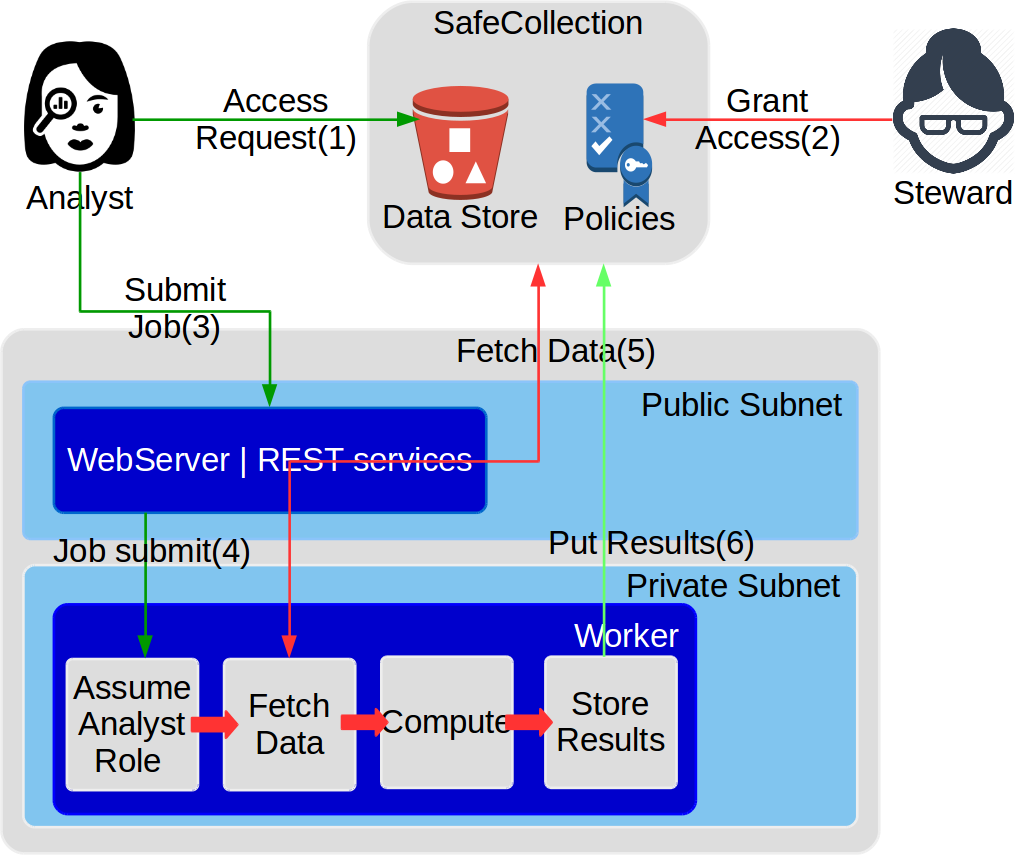
\includegraphics[width=0.45\textwidth]{figures/safe_flow.png}
  \caption{Safe collection schema}
  \label{fig:flow1}
  \vspace{-1.5em}
\end{figure}


\subsubsection{Export Flow}

Once Bob's analysis task is complete Bob realizes that he requires export approval before he may view the
results, so he issues a request to export his results. Alice, one of the collection's stewards, recieves
the export request on her dashboard. Alice assumes
the steward role with a fresh authenticated token, and accesses the results and the complete description
of Bob's analysis task. Alice reviews the data and the analysis to determine if the results are
safe for export. When she is satisfied with Bob's process, she initiates data export. \NAME
uses Alice's temporary credentials to transfer the results from the safe collection to a public
safe collection, accessible only to Bob, and updates the task information with new location of the results. Bob can now log on
and view or download the results. This flow is show in \figurename~\ref{fig:flow2}

\begin{figure}
  \center
  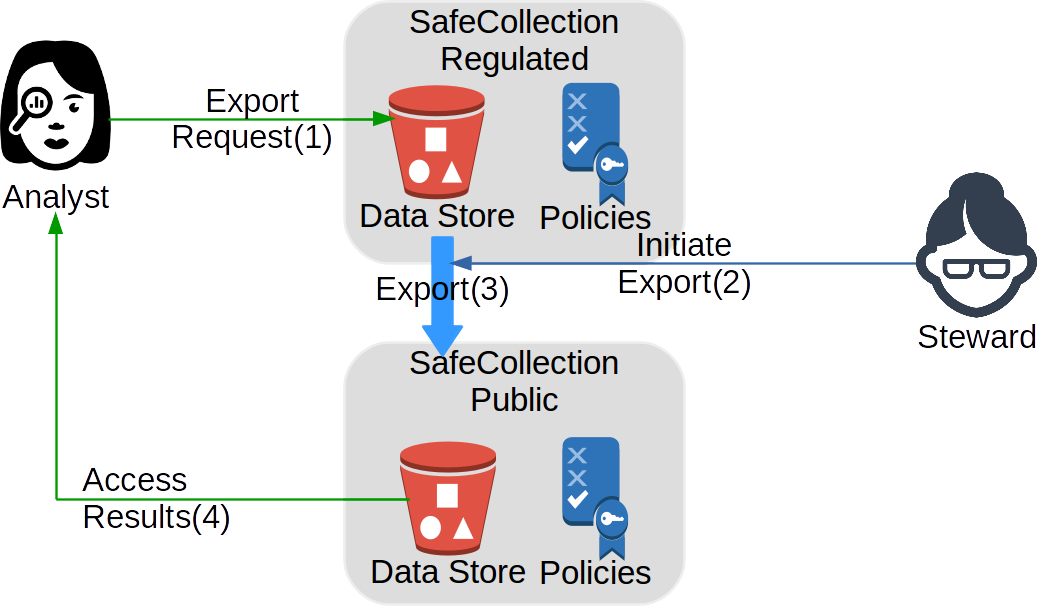
\includegraphics[width=0.45\textwidth]{figures/export_flow.png}
  \caption{Safe collection schema}
  \label{fig:flow2}
  \vspace{-1.5em}
\end{figure}



\section{Implementation}

The \NAME service is built upon a set of reliable and secure
AWS services. We extend this architecture to support safe collections
by building upon additional AWS capabilities and services. 

Safe collection policies are expressed on \NAMENS's managed
data via AWS Identity and Access Management (IAM) policies 
and S3 bucket policies.
A safe collection is described in CloudFormation templates, where 
CloudFormation provides a reproducible method for instantiating infrastructure
based on a standard JSON description. For example, it defines
the S3 bucket to be used as well as the secure connections
to the rest of the \NAME system.
\kyle{I dont understand exactly how CloudFormation describes the collection? Is
what I wrote correct?}
%This allows safe-collection descriptions to be verifiable, reproducible, and shareable.

To enable the definition and management of safe collection policies we 
rely on a meta-policy model. The meta-policy model enables specification
of the policies described above. Each safe collection is associated with a steward
(or group of stewards) who may manage the collection's policies. To simplify use, the meta-policy schema 
is translated to a web-based form that can be completed by users during creation of a safe collection. 
The defined policies (from the form or otherwise) is stored as a set of secure tags 
on the collection's data storage bucket. The schema is enforced
by the various services that interact with the safe collection. The schema and the generated form are shown in
\figurename~\ref{fig:schema}

\begin{figure*}[ht]
  \center
  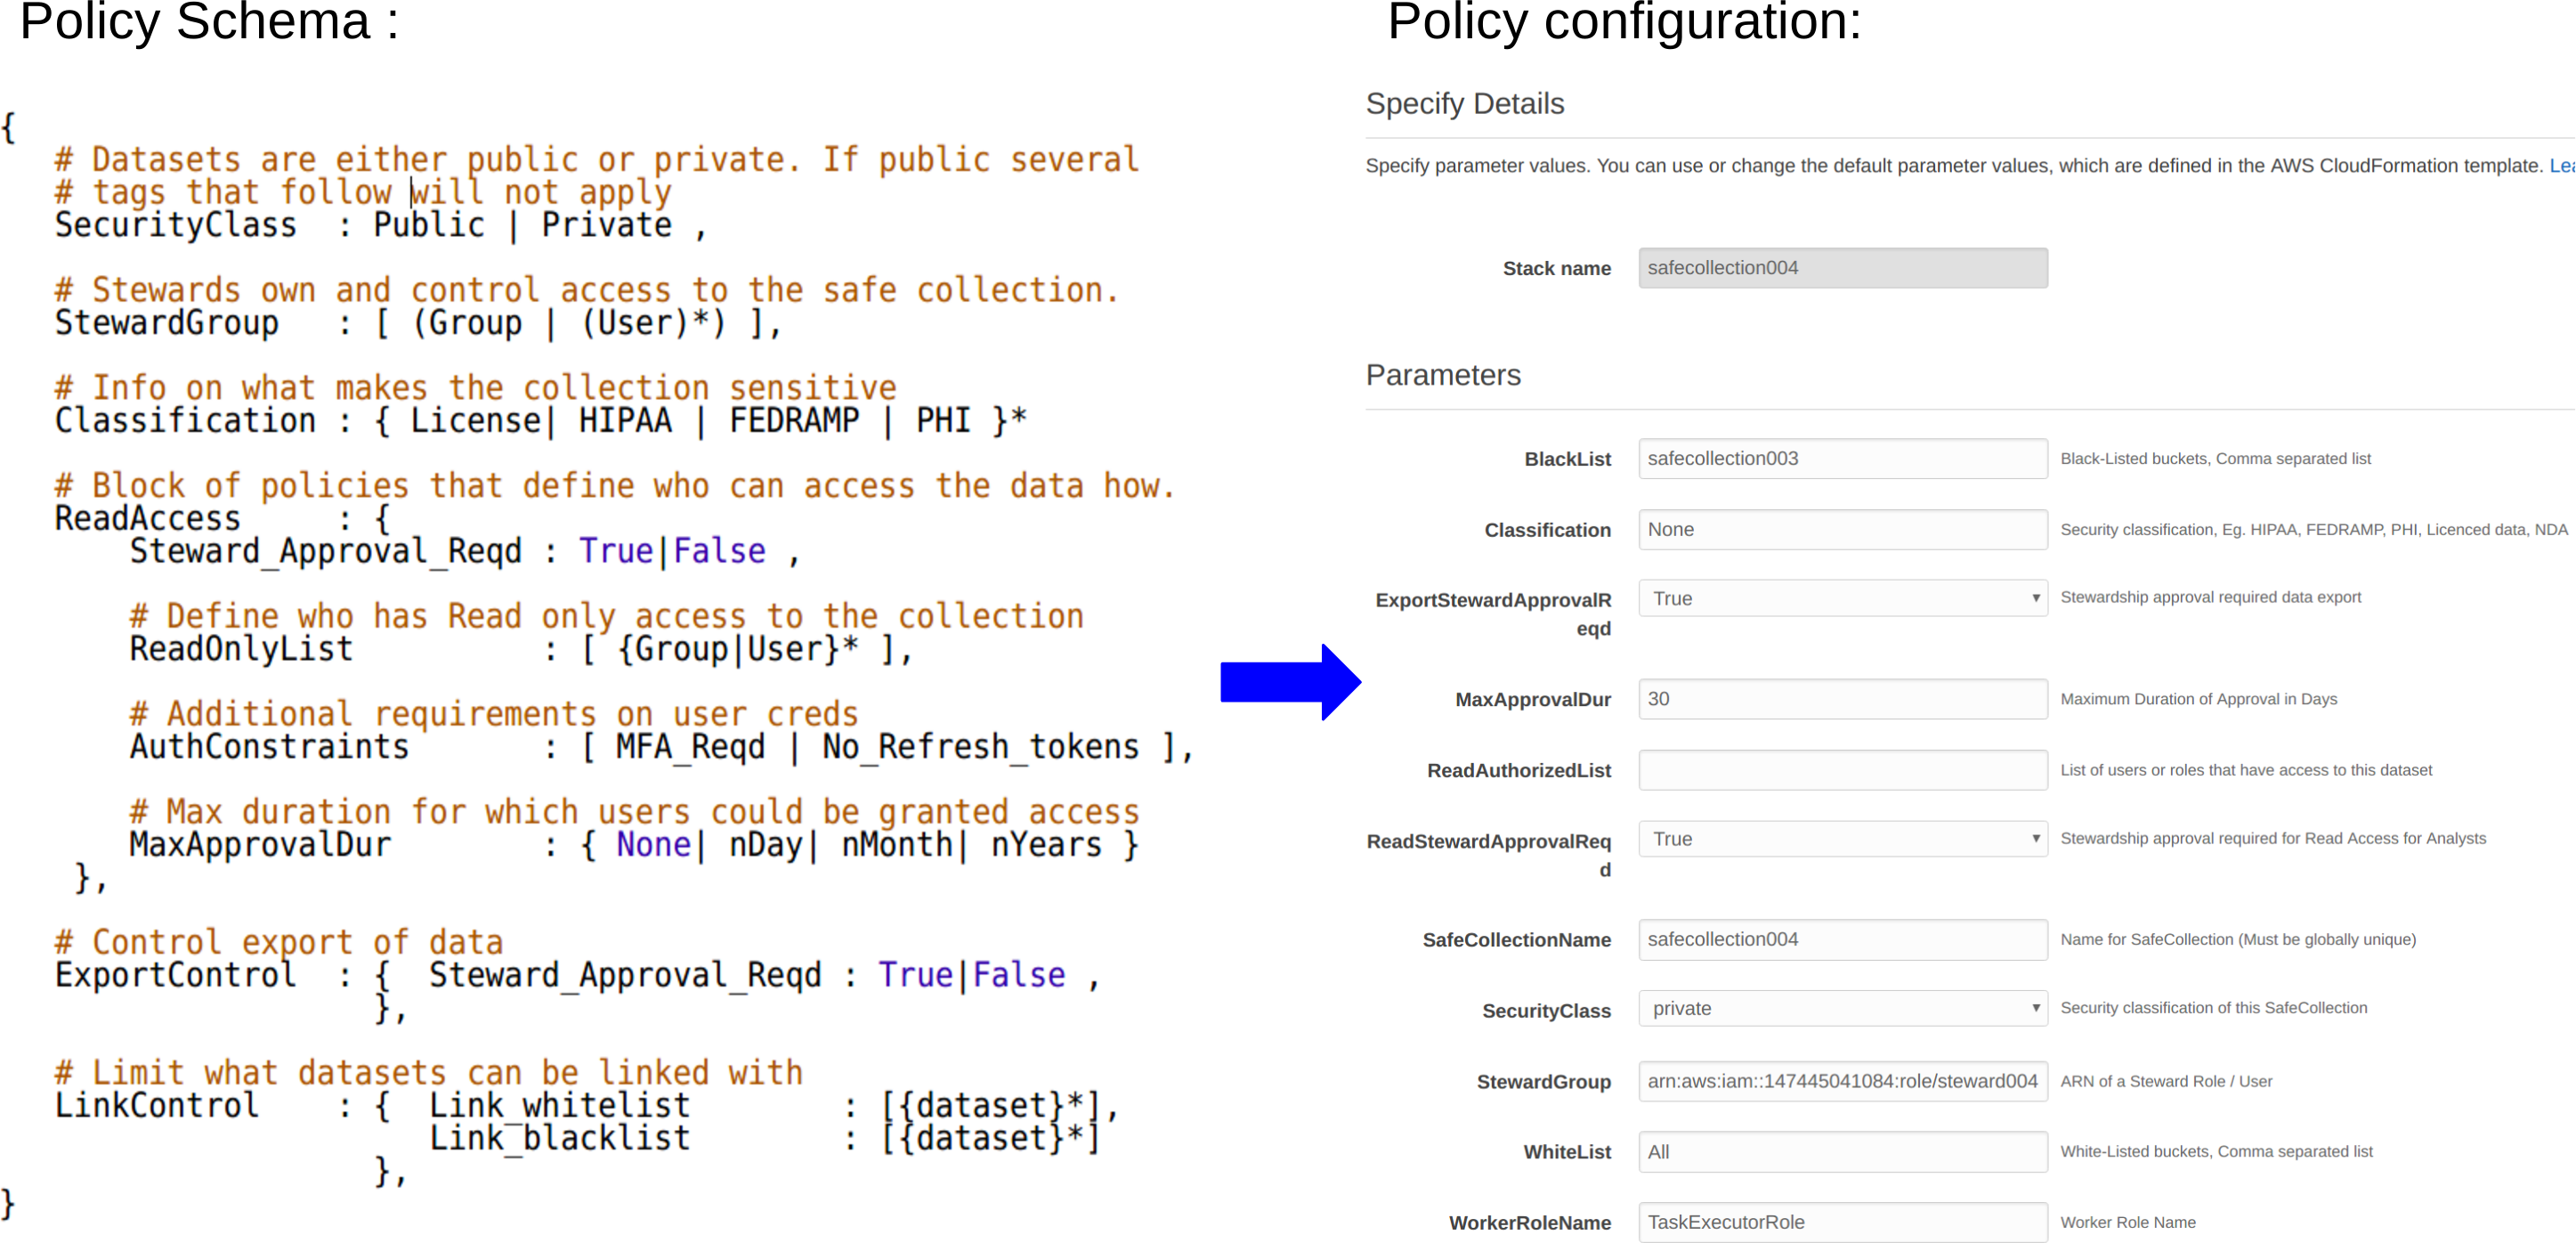
\includegraphics[width=\textwidth, height=8cm]{figures/meta-policy.png}
  \caption{Meta-policy specification and configuration}
  \vspace{-1.5em}
  \label{fig:schema}
\end{figure*}

Upon creation of a safe collection a single steward group (implemented as an IAM role) is added to the
access policies of the safe collection. This steward role is the sole entity on the platform capable of
updating policies attached to the safe collection.
Multiple users can be associated with the steward role---this is often recommended such 
that requests can be served quickly. 
Having established one's identity (via the \NAME authentication workflow) users 
may ``assume'' a privileged IAM role for which they are permitted. 
When assuming the steward role, a user temporarily gains the privileges to carry out operations such
as updating access policies and approving the export of data from a safe collection.

% implementation of access control
Access control on safe collections are managed by stewards. Access privileges for specific users
are granted, extended, and revoked via S3 bucket policies. At the time of creation all
privileges over bucket policies are granted to the steward and revoked for all other entities. This
guarantees that only the stewards can grant privileges on a safe collection. Access to other users 
is granted by stewards by adding a new bucket policy conditional on an expiration deadline. These policies may be revoked or
extended by updating the expiration deadline, thus offering fine-grained control to stewards for managing
access.

Data derived from safe collections (e.g., results from tasks that consumed data from that collection)
are stored in the same safe collection, thus inheriting the same policies as the safe collection itself.
As a result, only stewards can view the derived data and determine if it is safe to 
export the data
Stewards have complete visibility over all data that was used as input to an analysis as
well as the operations (analysis steps) made by the analysts to derive their results.
It is therefore possible to trace the entire provenance of the derived data from an
analysis pipeline since all analysis tasks are logged.
If an export request is approved, data is copied from the host collection to a public safe collection. 
It is important to note that even public safe collections have server side encryption and 
are only accessible to authenticated users via temporary signed URLs. 
As derived data are stored within the parent's safe collection, users can continue 
to perform analysis operations on results without oversight,
and only request export of data that must leave the safe collection (e.g., the
final results of a deep analysis pipeline).

Export approvals are implemented as a policy associated with the collection's bucket. 
\NAME ensures that the policy added is consistent with the meta-policy for the safe collection, 
for example, ensuring that expiration for the policy
is within the duration specified on the safe collection.

%On export controlled safe-collections, results generated by analysis tasks on \NAME are not visible to the
%analysts until approved by a Steward. This is implemented by having workers write all results to the
%parent safe-collections output directory and thus inheriting the same security privileges of the parent.





%\input{evaluation}
%\section{Related Work}

Secure data enclaves have a long and varied history starting with air gapped systems that are physically
disconnected from the internet.
While there are many examples of data enclaves, to the best of our knowledge none provide 
the stewardship and policy-based models used in \NAME. In this sections, we briefly review a range of data enclaves. 

NORC~\cite{lane2008using}, a research institution at the University of Chicago, operates a
data enclave to support researchers' investigations into programmatic, business, and policy decisions. 
NORC stores and manages a broad set of sensitive data in their FISMA compliant data enclave. The enclave
was designed with the vision of supporting multi-researcher collaboration via remote access terminals.
All microdata is hosted in a secure NORC server. 
This common approach to developing enclaves ensures security by access control, and limiting computation
to the server. However, it is limited by storage and computational infrastructure and the need to
host and operate local infrastructure. Moreover, it is typically not well
suited for large scale data analysis. Furthermore, users could potentially read microdata through 
their terminal. Thus, this approach only guarantees the privacy of the bulk of microdata.

The ICPSR data enclave \cite{icpsr} hosts sensitive datasets
for social science research. While the majority of the datasets are public, ICPSR
also manages restricted use datasets such as crime
data that are protected in data enclaves. They offer two types of data enclave: physical
and virtual. \kyle{Yadu - is this true?} The physical data enclave is a single protected server that is disconnected
from the internet and is accessible only in person. The virtual enclave is a remote desktop solution that is designed
to prevent copying of data. Systems such as these offer security at the cost of accessibility and ease of use while, at
the same time, lacking a solution to the fundamental problem of users manually copying sensitive microdata records.

The National Center for Health Statistics (NCHS) Research Data Center (RDC) \cite{cdc} hosts a large collection of
restricted datasets. These datasets contain health information and are subject to HIPAA guidelines.
The data is accessible on-premise at the NCHS RDC or the Federal Statistical RDC, or in some
cases via remote access. 
%several datasets are not available for remote access. 
RDC restricts access to direct identifiers such as name and 
social security number while leaving indirect identifiers such as geography accessible. Even with the constraints
on access and limited record accessibility, access to potentially identifying information leaves this system open to
linkage attacks. This is mitigated, to some extent, by strong vetting of research proposals.

The NCI Genomic Data Commons \cite{grossman2016toward} hosts several Petabytes of
genomic data, and provides an on-premise cloud model to enable computation on these sensitive datasets.
While the on-premise infrastructure meets compliance requirements, this choice leads to added costs associated with
building and maintaining production compute infrastructure---an approach that is unlikely to be 
broadly available to a wide range of scientists. \NAME, and other cloud-based enclaves, benefit
significantly from the low-cost cloud resources made possible due to providers' economies of scale.





%


There are significant opportunities for new scientific discoveries to be made
through the collaborative analysis of sensitive and protected
data.  While many approaches to storing such data
have been adopted in production deployments, in most cases there are
considerable barriers that overly restrict data access and analysis. 
Importantly, there is little ability for dataset owners and administrators
to define and apply sophisticated administrative models and policies 
for securely managing that data. 

To address these concerns we have developed two important abstractions
that allow data owners to securely manage data in ways that permit
controlled access and analysis. The secure collection provides a 
policy-based approach for defining the interactions with a particular
dataset. Data stewards are associated with collections to then
manage the collection and review the actions of users. These
constructs have been implemented in the \NAME data enclave
and have since been adopted to protect a range of sensitive
social science data. Initial experiences with the model
have been positive, with data owners valuing the ability 
to securely manage collections, and users valuing the clearly
defined policies for data access and analysis. 

%\section{Availability}

%\yadu{Add notes on the github page about how to deploy} % I'd omit this for this shorter paper // AG



\section*{Acknowledgments}
Ack - Klab, DSaPP, Tristan
%% Should we still ack Templeton? // AG

%\yadu{Pete Aceves did some testing for the security stuff}
% trigger a \newpage just before the given reference
% number - used to balance the columns on the last page
% adjust value as needed - may need to be readjusted if
% the document is modified later
%\newpage
%\IEEEtriggeratref{8}

% The "triggered" command can be changed if desired:
%\IEEEtriggercmd{\enlargethispage{-5in}}

% references section

% can use a bibliography generated by BibTeX as a .bbl file
% BibTeX documentation can be easily obtained at:
% http://mirror.ctan.org/biblio/bibtex/contrib/doc/
% The IEEEtran BibTeX style support page is at:
% http://www.michaelshell.org/tex/ieeetran/bibtex/
\bibliographystyle{IEEEtran}
% argument is your BibTeX string definitions and bibliography database(s)
\bibliography{references}
%
% <OR> manually copy in the resultant .bbl file
% set second argument of \begin to the number of references
% (used to reserve space for the reference number labels box)

% that's all folks
\end{document}


